\documentclass[fontset=windows]{article}
\usepackage[margin=1in]{geometry}
\usepackage{ctex}
\usepackage{setspace}
\usepackage{lipsum}
\usepackage{graphicx}
\usepackage{caption}
\usepackage{subcaption}
\usepackage[colorlinks=true,linkcolor=red]{hyperref}

\graphicspath{{figures/}}

\title{\heiti\zihao{2} Common-Gate Stage}
\author{\songti zrrraa}
\date{2023.12.18}

\begin{document}
\maketitle
\thispagestyle{empty}

\section*{Small-Signal Properties}

We assume that $\lambda=0$. 

\begin{figure}[htbp]
    \centering
    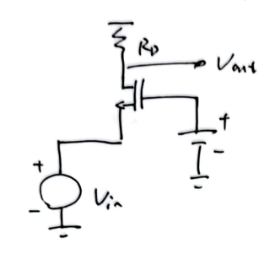
\includegraphics[scale=0.8]{1.jpg}
    \captionsetup{labelformat=empty}
    \caption{}
    \label{1}
\end{figure}

Convert circuit model to small signal model. 

\begin{figure}[htbp]
    \centering
    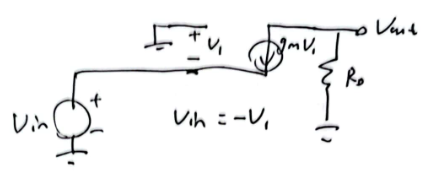
\includegraphics[scale=0.8]{2.jpg}
    \captionsetup{labelformat=empty}
    \caption{}
    \label{2}
\end{figure}

We get: 

$$\frac{v_{out}}{R_D}=-g_mv_1=g_mv_{in}\Longrightarrow A_v=g_mR_D$$

\subsection*{Input Impedance}

Next we calculate the input and output impedance. 

\begin{figure}[htbp]
    \centering
    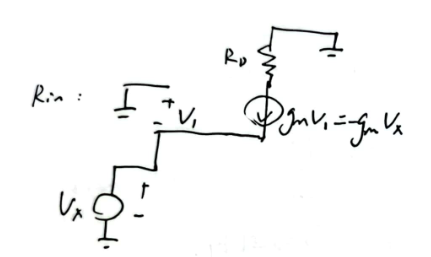
\includegraphics[scale=0.8]{3.jpg}
    \captionsetup{labelformat=empty}
    \caption{}
    \label{3}
\end{figure}

$$i_x=g_mv_x\Longrightarrow R_{in}=\frac{1}{g_m}$$

$g_m$ is usually around tens to hundreds, which means that the input impedance of the common gate amplifier is very low. 
Such low impedance can be used for impedance matching of antennas and other devices. 

\begin{figure}[htbp]
    \centering
    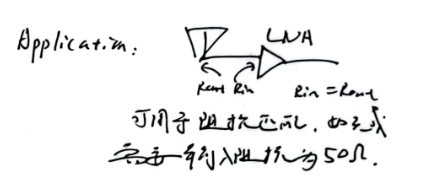
\includegraphics[scale=0.8]{4.jpg}
    \captionsetup{labelformat=empty}
    \caption{}
    \label{4}
\end{figure}

\subsection*{Output Impedance}

\begin{figure}[htbp]
    \centering
    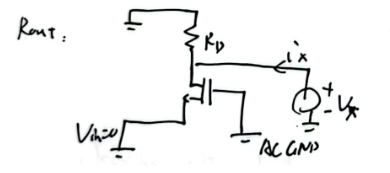
\includegraphics[scale=0.8]{5.jpg}
    \captionsetup{labelformat=empty}
    \caption{}
    \label{5}
\end{figure}

We get: 

$$R_{out}=R_D$$

\section*{Example}

\begin{figure}[htbp]
    \centering
    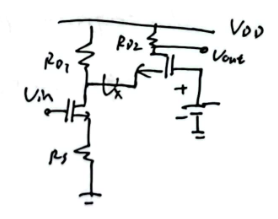
\includegraphics[scale=0.8]{6.jpg}
    \captionsetup{labelformat=empty}
    \caption{}
    \label{6}
\end{figure}

$$\frac{V_{out}}{V_{in}}=\frac{V_x}{V_{in}}\frac{V_{out}}{V_x}$$

Because: 

$$\frac{V_x}{V_{in}}=-\frac{R\ tied\ between\ AC\ Ground\ and\ Drain}{\frac{1}{g_m}+R\ tied\ between\ Source\ and\ AC\ Ground}$$

We can derive: 

$$\frac{V_{out}}{V_{in}}=-\frac{R_{D1}||\frac{1}{g_{m1}}}{\frac{1}{g_{m1}}+R_S}g_{m2}R_{D2}$$

\subsubsection*{Output Resistance of CG Stage in a Special Case}

Now we assume $\lambda \neq 0$

\begin{figure}[htbp]
    \centering
    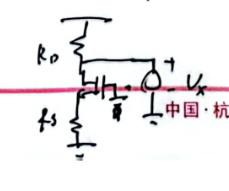
\includegraphics[scale=0.8]{7.jpg}
    \captionsetup{labelformat=empty}
    \caption{}
    \label{7}
\end{figure}

Use the conclusions you reached last time, we get: 

$$R_{out}=R_D||[(1+g_mr_o)R_s+r_o]$$

\section*{Bias Design}

\begin{figure}[htbp]
    \centering
    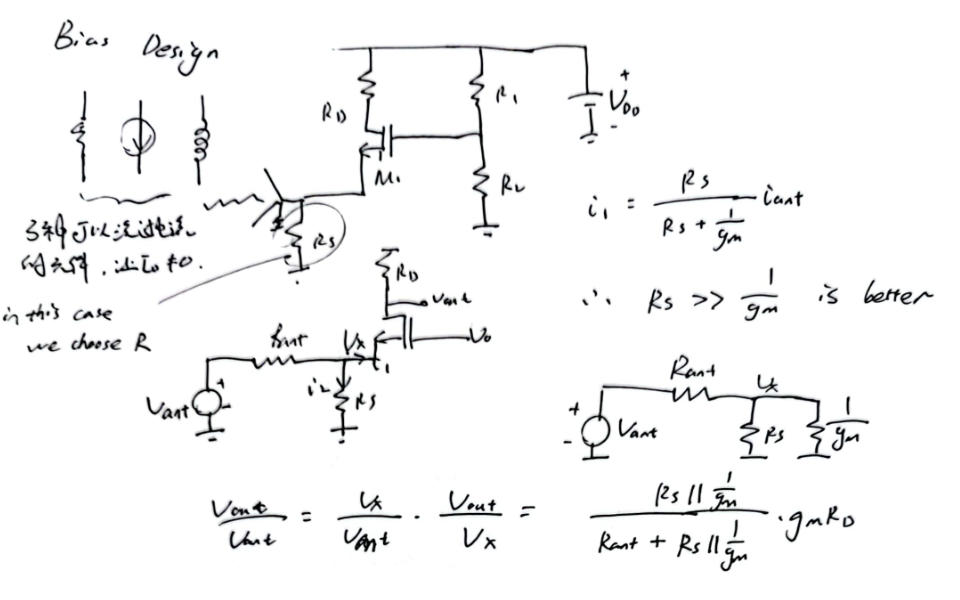
\includegraphics[scale=0.8]{8.jpg}
    \captionsetup{labelformat=empty}
    \caption{}
    \label{8}
\end{figure}

Use a resistor to ensure $I_D \neq 0$. 

$$i_1=\frac{R_s}{R_s+\frac{1}{g_m}}i_{out}$$

So if we want more signal to go into the common gate amplifier instead of being consumed by the resistor, we should ensure that: 

$$R_s>>\frac{1}{g_m}$$

We can also calculate the $V_out$ using the input impedance. 

$$\frac{V_{out}}{V_{ant}}=\frac{V_x}{V_{ant}}\frac{V_{out}}{V_x}=\frac{R_s||\frac{1}{g_m}}{R_{out}+R_s||\frac{1}{g_m}}*g_mR_D$$

\section*{Example}

\begin{figure}[htbp]
    \centering
    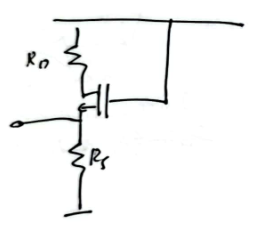
\includegraphics[scale=0.8]{9.jpg}
    \captionsetup{labelformat=empty}
    \caption{}
    \label{9}
\end{figure}

In actual situations, due to the need to ensure that the MOSFET works in the saturation region, we may not necessarily be able to satisfy that $R_s$ is much greater than $\frac{1}{g_m}$. 

In this case, $R_{smax}=\frac{V_{DD}-V_{GS}}{I_D}=370\Omega$

Ensure that $I_DR_D\leq V_{TH}$, we choose $R_D=500\Omega$. 

Then we can calculate $A_v=1.6$. 

If double $\frac{W}{L}$, $A_v=2.3$, but the capacitance will also become larger, leading to the drop of the speed. 

\section*{Link}

\href{https://www.bilibili.com/video/BV1FD4y1R7Ah?p=40&vd_source=1d0c07486a3bd3b0adb8ac548bf6453e}{Razavi Electronics Circuits 1: lectrue 40}
\end{document}